\section{Conjunto de Datos}
En este apartado se describe el conjunto de datos empleado para el entrenamiento del modelo de árbol de decisión, diseñado con el objetivo de detectar posibles comunicaciones asociadas a ransomware.

El conjunto de datos utilizado proviene del trabajo realizado por Eduardo Berrueta et al. entre los años 2015 y 2022\cite{qnyn-q136-20}. Este dataset contiene capturas de tráfico en formato .pcap correspondientes a setenta familias distintas de ransomware, con un volumen total superior a 60 GB con los datos comprimidos.

Debido a las limitaciones de almacenamiento y capacidad de cómputo disponibles, así como al alcance definido para este trabajo, he optado por trabajar únicamente con dos de las muestras incluidas en el conjunto de datos original, que serán los que trataremos en profundidad en este apartado.

Pero antes de tratar estos dos subconjuntos de datos en concreto, cabe hacer una mención al artículo de Eduardo Berrueta y su equipo\cite{9050526}. En él explican que la motivación para crear el dataset proviene de la necesidad de estandarizar recursos a la hora de evaluar la fiabilidad de las herramientas de detección de ransomware, ya que habitualmente cada fabricante o investigador utiliza su propio conjunto de datos. Al ser estos conjuntos muy específicos y reducidos, las comparativas resultantes tienden a ser poco realistas. Con su trabajo, Berrueta pretende aportar un dataset completo para pruebas de detección de ransomware que contribuya a resolver estas problemáticas.

Para este trabajo he usado muestras de dos ransomwares tomadas en el año 2021. El primero de los casos analizados es Hive, un conocido Ransomware-as-a-Service (RaaS) que emergió en junio de 2021. Este ransomware se caracterizaba por emplear un esquema de cifrado híbrido basado en los algoritmos RSA y AES, y por implementar una estrategia de doble extorsión. En este modelo, no solo se cifraban los datos de la víctima, sino que también se exfiltraban, exigiendo posteriormente un pago tanto por la clave de descifrado como por evitar la publicación de la información sustraída\cite{KIM2022103387}. El segundo de los casos analizados es CryLock, una variante evolucionada del ransomware Cryakl. CryLock se propagaba principalmente a través de correos electrónicos de phishing o campañas de spam, y al igual que otros ransomware modernos, empleaba un esquema de cifrado híbrido basado en los algoritmos RSA y AES. Además, una de sus características distintivas era la eliminación de las copias de seguridad presentes en los dispositivos comprometidos, con el objetivo de dificultar la recuperación de los datos sin realizar el pago del rescate.\cite{HeimdalCryLock2022}

\section{Métodos de Filtrado de Paquetes}
El filtrado de paquetes constituye una de las técnicas fundamentales para el control del tráfico en redes informáticas. Su propósito principal es inspeccionar, permitir o bloquear paquetes de datos en función de criterios previamente definidos, como direcciones IP, puertos, protocolos o patrones de comportamiento. 

A lo largo de la evolución de las redes de comunicaciones, el problema del filtrado de paquetes ha sido abordado mediante una amplia variedad de enfoques, que van desde soluciones sencillas y de rápida implementación hasta mecanismos con un alto grado de complejidad técnica. El mecanismo más sencillo de implementar para el filtrado de paquetes es el uso de un firewall. En los sistemas operativos GNU/Linux, este puede configurarse mediante el comando iptables, que opera a través de Netfilter, el subsistema encargado del filtrado de paquetes a nivel de kernel. El hecho de que el firewall funcione en espacio de kernel permite que su impacto sobre el rendimiento del sistema sea reducido. Su función principal consiste en controlar el tratamiento de los paquetes de red entrantes, salientes y reenviados, permitiendo aceptarlos, denegarlos, redirigirlos o registrarlos en función de criterios como dirección IP, puertos, protocolos, entre otros.\cite{LinuxIptables}

Otro enfoque relevante para el filtrado de paquetes, especialmente orientado a la seguridad de los sistemas, es el uso de sistemas de detección de intrusiones (Intrusion Detection Systems, IDS por sus siglas en inglés). Uno de los más reconocidos en este ámbito es Snort, ampliamente utilizado desde su lanzamiento en 1998 y caracterizado por ser de código abierto\cite{Roesch1999Snort}. Para llevar a cabo el filtrado, Snort emplea la biblioteca libpcap para capturar paquetes de red, que posteriormente son decodificados para identificar su estructura y los protocolos involucrados (Ethernet, IP, TCP/UDP, entre otros). A partir de esta información, Snort monitoriza el tráfico y genera alertas en función de un conjunto de reglas predefinidas. Además, este sistema puede operar en diferentes modos: sniffer, logger o como IDS propiamente dicho, y permite su ampliación mediante un sistema de plugins.

Esta evolución desde mecanismos de filtrado simples hacia un análisis más profundo del tráfico se ha visto respaldada por tecnologías como libpcap y BPF (Berkeley Packet Filter), que permiten la captura eficiente de paquetes sin comprometer significativamente el rendimiento del sistema. BPF es una interfaz que habilita la captura de paquetes a través de programas escritos en lenguaje C, los cuales deben ajustarse a un conjunto de restricciones más estricto que el lenguaje C estándar. Un aspecto clave de BPF es su modelo de ejecución: aunque los filtros se definen desde el espacio de usuario, su ejecución se realiza en el espacio del kernel, lo que permite un procesamiento más rápido y eficiente al evitar cambios de contexto innecesarios\cite{FreeBSDBPF}.

Por otro lado, libpcap es una biblioteca inicialmente desarrollada en C, que actualmente cuenta con una versión en Python, y que se utiliza para capturar paquetes ofreciendo una API uniforme para acceder a datos de red a bajo nivel desde el espacio de usuario. Cuando el sistema lo permite, libpcap hace uso de BPF para realizar filtrado a nivel de kernel\cite{LibpcapDocs2025}. Esta biblioteca (y, por extensión, BPF) ha sido utilizada en multitud de herramientas, entre ellas Wireshark\cite{WiresharkLibpcapWiki}.

BPF ha ido evolucionando a lo largo de los años, llegando su desarrollo hasta eBPF (Extended Berkeley Packet Filter). eBPF, como su propio nombre indica, comenzó siendo una extensión de BPF, pero con el paso del tiempo se ha convertido en una plataforma más general capaz de interactuar con distintas partes del sistema operativo, tales como redes, seguridad, trazado y observabilidad. A diferencia del BPF original —que únicamente filtraba paquetes en el espacio del socket—, eBPF permite engancharse (hook) en múltiples puntos del kernel, ejecutar programas verificados para garantizar la seguridad, utilizar mapas compartidos entre el kernel y el espacio de usuario, y beneficiarse de la compilación JIT (Just In Time) para un alto rendimiento\cite{ebpf_website}. En base a eBPF, se ha desarrollado XDP (eXpress Data Path), una tecnología para el kernel de Linux que permite ejecutar programas eBPF en una etapa más temprana del procesamiento de paquetes, lo que se traduce en una menor latencia y un mayor rendimiento. Para ello, XDP establece como hook el controlador (driver) de la tarjeta de red, o bien opera en modos alternativos como generic (pila de red) u offload (hardware si la NIC lo soporta). De este modo, el filtrado de paquetes se sitúa en la capa más baja de la pila de red. Es importante señalar que XDP requiere especificar la tarjeta de red sobre la que se ejecutará el programa eBPF\cite{AyaXDP}.

Para entender lo que resta del presente trabajo es necesario entender el flujo de funcionamiento de XDP y por lo tanto es necesario conocer el flujo de eBPF, para ello nos basaremos en \ref{ebpf-workflow} obtenido de\cite{ebpf_website}. El primer paso consiste en escribir el programa en un subconjunto restringido del lenguaje C. Posteriormente, mediante herramientas como Clang y LLVM, el código se compila a bytecode. A continuación, desde el espacio de usuario, el programa se carga en el espacio del kernel y se prepara el espacio de usuario para recibir información mediante los mapas definidos en el programa, en caso de ser necesario. Estos dos últimos pasos pueden realizarse mediante un programa en C en el espacio de usuario utilizando la biblioteca libbpf. Una vez que el programa llega al kernel, este pasa por el verificador, cuyo objetivo es impedir la ejecución de acciones no permitidas, como bucles infinitos o accesos ilegales a memoria. A continuación, el compilador en tiempo real (Just-In-Time compiler, JIT) transforma el bytecode en código máquina. Tras este proceso, el programa se “engancha” (hook) a diferentes eventos de la capa de red, como, por ejemplo, el controlador (driver) de la tarjeta de red en el caso de XDP. Durante la ejecución, y siempre que sea necesario, el programa interactúa con los mapas definidos. Este flujo garantiza que el código eBPF se ejecute de forma segura y eficiente, integrándose de manera controlada en el sistema operativo.

\begin{figure}[Flujo eBPF]{ebpf-workflow}{Flujo de ejecución de un programa eBPF. Obtenida de\cite{ebpf_website} siguiendo la licencia Creative Commons Attribution 4.0 International License.}
	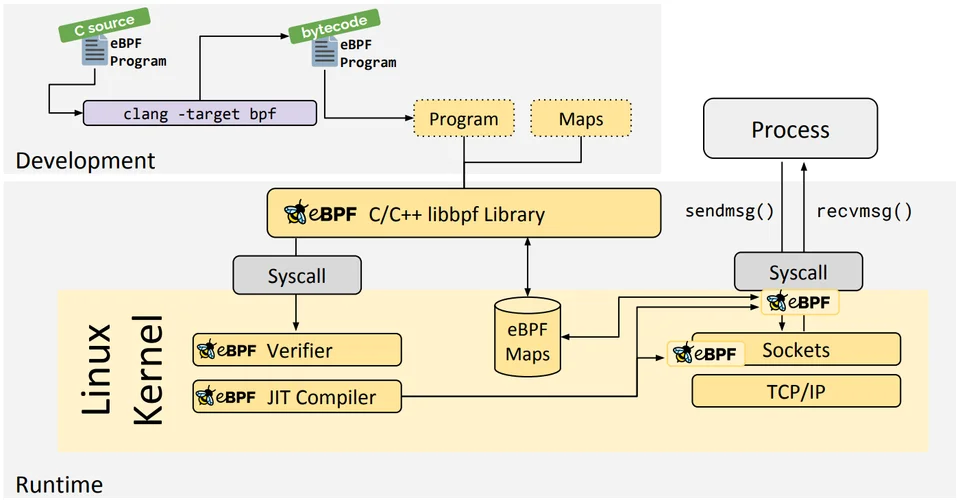
\includegraphics[width=0.9\textwidth]{capturas/eBPF_workflow.png}
\end{figure}

\section{Artículos Similares y Relacionados}
Como se ha expuesto en la motivación y en las subsecciones anteriores, la detección temprana de ransomware y la necesidad de contar con sistemas de filtrado de paquetes que ofrezcan un alto rendimiento y una baja latencia constituyen problemáticas que han captado la atención y el interés de la comunidad académica desde hace tiempo. Dado que el presente trabajo se centra en analizar el impacto en el rendimiento de red de sistemas de detección y filtrado de ransomware basados en árboles de decisión, resulta pertinente revisar los trabajos académicos que exploran tanto el uso de tecnologías como eBPF y XDP en el filtrado de tráfico malicioso, como aquellos que estudian la aplicación de árboles de decisión para la detección de ransomware.
